\hypertarget{convdiff01_8cpp}{
\subsection{/home/luiggi/Documents/Research/Meshless\_\-RBF/NEW/RBFSoft/examples/04ConvDiff1D/convdiff01.cpp File Reference}
\label{convdiff01_8cpp}\index{/home/luiggi/Documents/Research/Meshless\_\-RBF/NEW/RBFSoft/examples/04ConvDiff1D/convdiff01.cpp@{/home/luiggi/Documents/Research/Meshless\_\-RBF/NEW/RBFSoft/examples/04ConvDiff1D/convdiff01.cpp}}
}
Non-stat adv-diff equation in 1D.  




\subsubsection{Detailed Description}
Non-stat adv-diff equation in 1D. 

In this example the time-dependent advection-diffusion equation in 1D is solved. The equation is written as follows: \[ \frac{\partial f}{\partial t} + u \frac{\partial f}{\partial x} - D \frac{\partial^2 f}{\partial x^2} = 0 \] where $u$ represents a convective velocity. The initial and boundary conditions are: \begin{eqnarray*} f(x,0) & = & 0 \textrm{ for } 0 \le x < \infty, \\ f(0,t) & = & 1 \textrm{ for } t \ge 0, \\ f(L,t) & = & 0 \textrm{ for } t > 0, L \rightarrow \infty, \end{eqnarray*}  \begin{Image}
\begin{center}
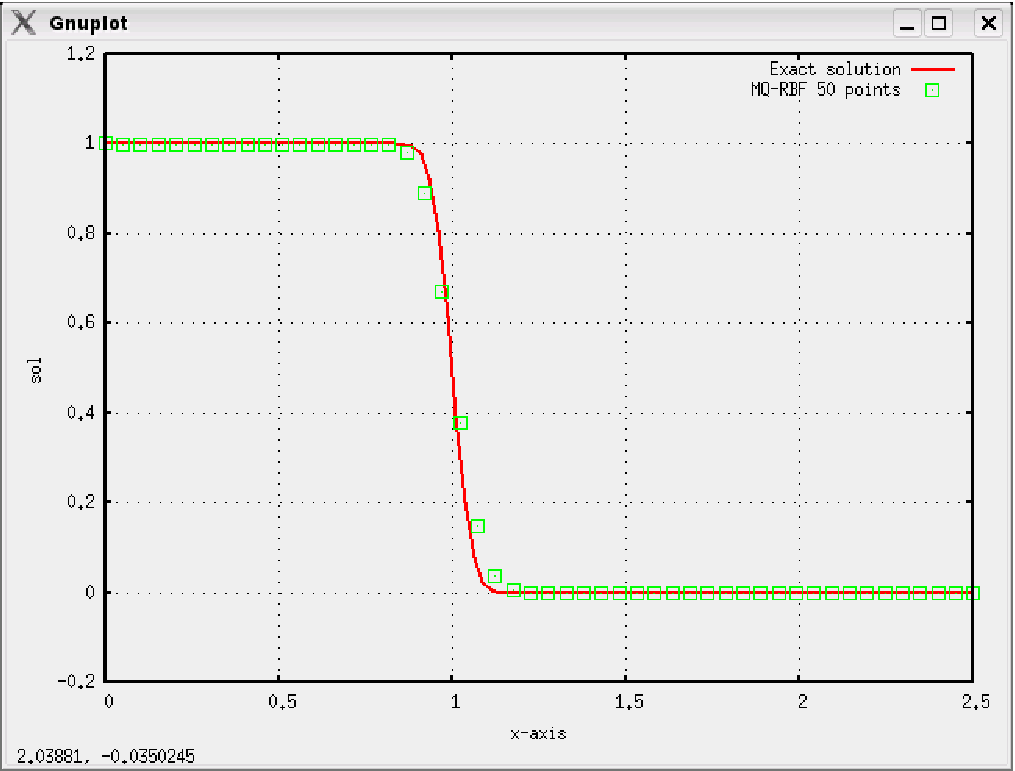
\includegraphics[width=5cm]{soladvdiff1D}\caption{MQ-RBF solution for D = 0.0001 and 50 points}
\end{center}
\end{Image}
 \begin{Desc}
\item[Input]The {\tt input} file contains the initial data to setup the problem:\begin{itemize}
\item {\tt h} lenght of the domain\item {\tt N} number of points\item {\tt max\_\-iter} max time iterations\item {\tt dt} time step\item {\tt D} Peclet number\item {\tt max\_\-knots} neighbor knots for the ACBF precond. \end{itemize}
\end{Desc}
\begin{Desc}
\item[Output]\begin{itemize}
\item {\tt xy\_\-knots.dat} x-coordinates of the points.\item {\tt solution.dat} evaluation of the final solution.\item {\tt error.dat} error against the exact solution.\item {\tt exact.dat} exact solution.\end{itemize}
\end{Desc}
\begin{Desc}
\item[Author:]Luis M. de la Cruz \mbox{[} Thu Sep 6 14:35:41 BST 2007 \mbox{]} \end{Desc}


Definition in file \hyperlink{convdiff01_8cpp-source}{convdiff01.cpp}.